% ====================================================================
%  Chapter: Digital Twin
% ====================================================================
\newpage
\section{Digital Twin and Real-Time Smart Home Map}
\label{sec:digital-twin}

This section describes the digital-twin layer of H.E.R.A. In this project, the digital twin is not a purely decorative floor-plan screen. It is a live cyber-physical representation of the house: physical telemetry from the ESP32 is streamed upward through MQTT and backend APIs, transformed into normalized device and sensor state, and projected onto an interactive spatial map in the React dashboard. The user can inspect the state of each room, observe whether telemetry is fresh or stale, and send control commands from the map back to the physical devices.

\subsection{Digital Twin Rationale}

The main purpose of the digital twin is to close the interpretation gap between raw IoT data and resident understanding. A raw telemetry payload can show that \texttt{neo\_led.status=true}, \texttt{dht20.temperature=31.5}, or \texttt{mini\_fan.speed=512}, but these values do not immediately explain where the event occurs in the house or which physical object is affected. The digital twin solves this problem by binding every sensor and actuator to a room-level coordinate on the home layout. As a result, the user sees the smart-home state as a spatial environment rather than as isolated database fields.

This design also supports safer control. When a user clicks a device marker, the command is tied to a specific runtime target such as \texttt{main\_led}, \texttt{neo\_led}, \texttt{ws2812}, \texttt{mini\_fan}, or \texttt{relay}. The dashboard does not invent its own local device state. Instead, it sends control requests to the backend runtime and waits for telemetry confirmation. If telemetry becomes stale, the interface disables controls to avoid presenting outdated physical state as current truth.

\subsection{Frontend Implementation}

The digital twin is implemented in the React dashboard under \texttt{FE/hera-dashboard}. The core component is \texttt{FloorPlan.jsx}. It renders the house floor-plan image, overlays device and sensor markers at fixed percentage coordinates, subscribes to live telemetry, and updates the marker state whenever new data arrives.

\begin{figure}[H]
    \centering
    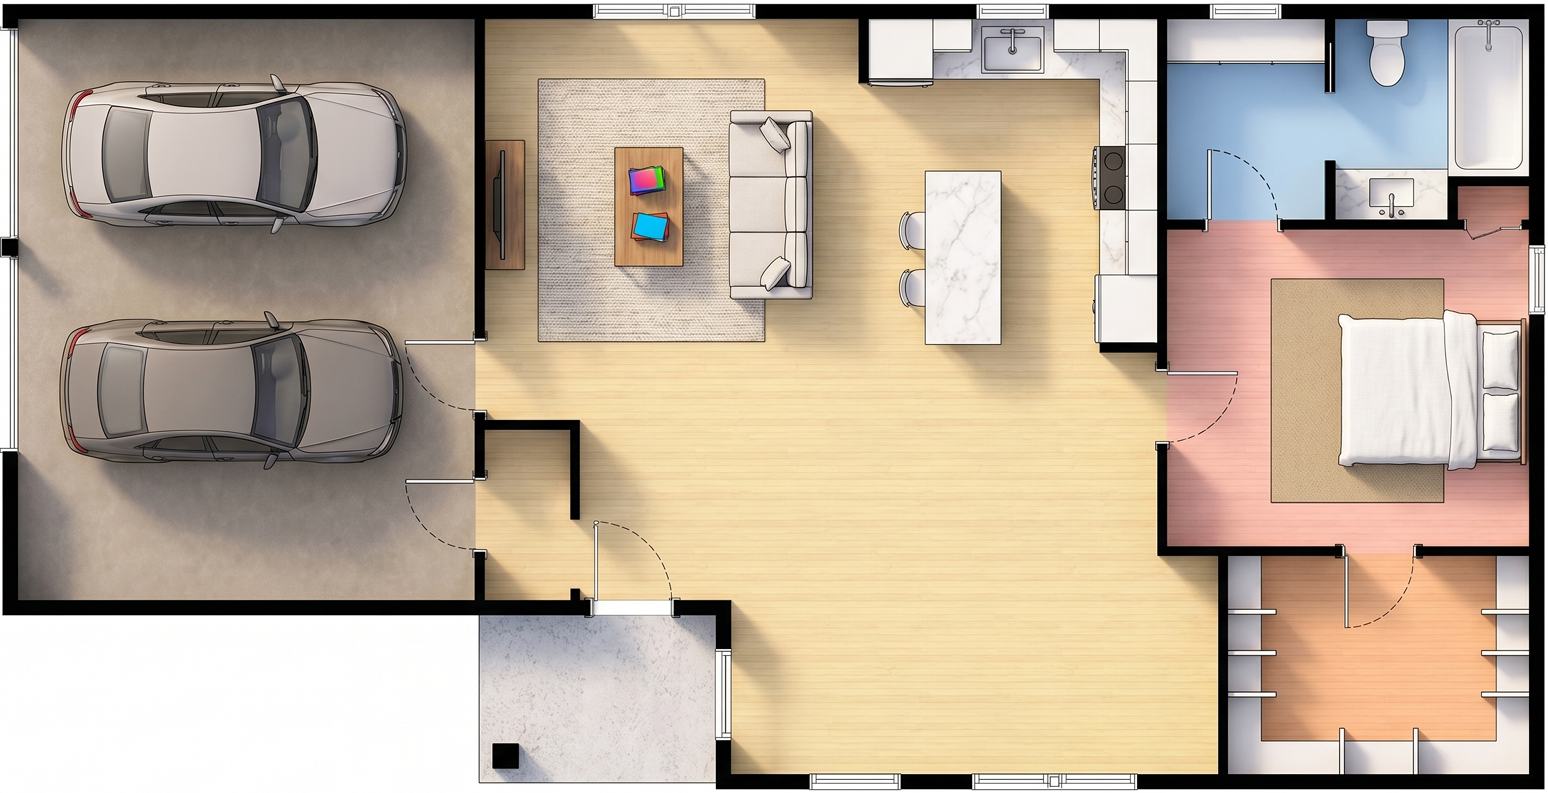
\includegraphics[width=0.95\textwidth]{image/digital_twin_floor_plan.png}
    \caption{House floor-plan asset used as the spatial base of the H.E.R.A digital twin.}
    \label{fig:digital-twin-floor-plan}
\end{figure}

\begin{figure}[H]
    \centering
    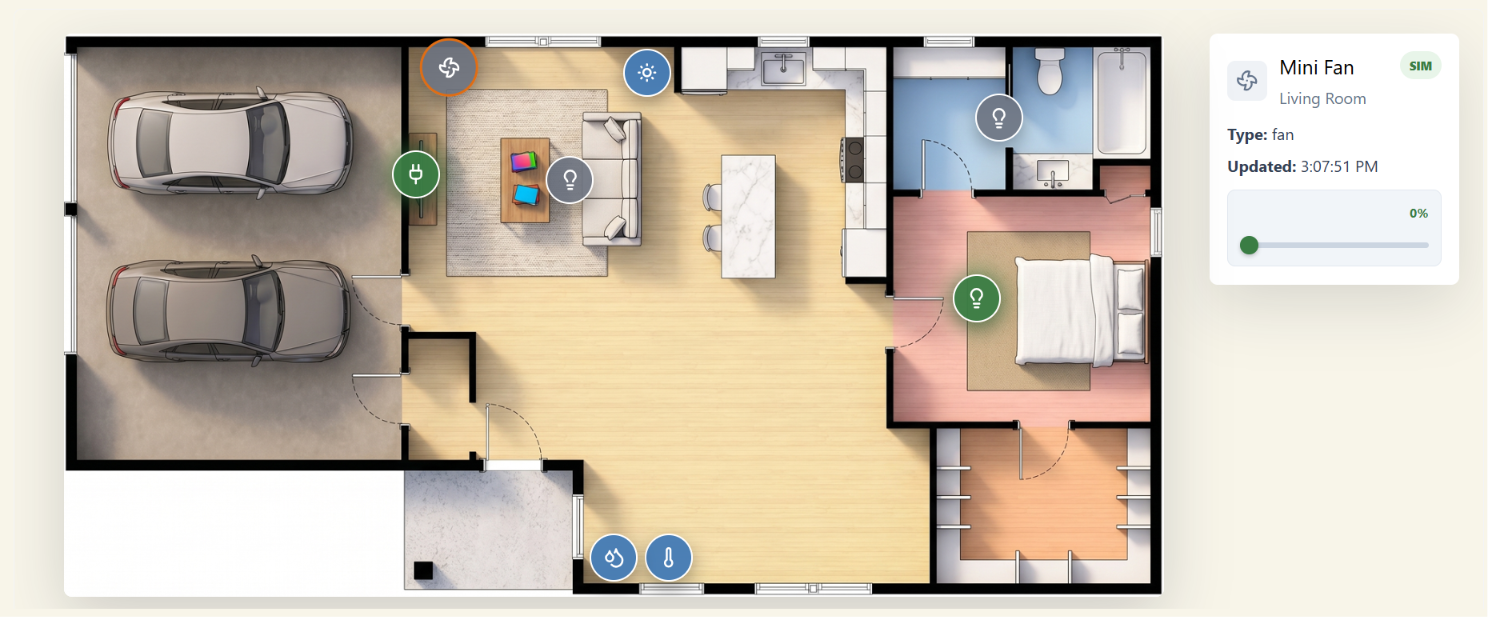
\includegraphics[width=0.95\textwidth]{image/UI/house.png}
    \caption{Implemented H.E.R.A house view with live device and sensor markers overlaid on the floor plan.}
    \label{fig:digital-twin-house-ui}
\end{figure}

The frontend marker catalog defines the semantic mapping between the visual map and the runtime system. Each marker contains an identifier, room name, device or sensor type, coordinate position, target identifier, and icon type. Table~\ref{tab:digital-twin-marker-map} summarizes the currently implemented map.

\begin{table}[H]
    \centering
    \caption{Digital-twin marker mapping in the React floor-plan component}
    \label{tab:digital-twin-marker-map}
    \renewcommand{\arraystretch}{1.16}
    \small
    \begin{tabularx}{\textwidth}{@{}p{2.4cm}p{2.5cm}p{2.4cm}p{2.2cm}X@{}}
        \toprule
        \textbf{Marker ID} & \textbf{Displayed object} & \textbf{Room} & \textbf{Runtime key} & \textbf{Twin behavior} \\
        \midrule
        \texttt{main\_led} & LED & Living Room & \texttt{main\_led} & Shows on/off state and sends lighting commands. \\
        \texttt{neo\_led} & LED & Bedroom & \texttt{neo\_led} & Shows on/off state and supports brightness control. \\
        \texttt{ws2812} & LED & Toilet & \texttt{ws2812} & Shows on/off state and supports brightness/color-related runtime control. \\
        \texttt{Fan} & Mini Fan & Living Room & \texttt{mini\_fan} & Shows fan state and supports speed-related control. \\
        \texttt{relay} & TV & Living Room & \texttt{relay} & Shows relay state and sends relay on/off commands. \\
        \texttt{temperature} & Temperature & Living Room & \texttt{temperature} & Displays the latest DHT20 temperature value. \\
        \texttt{humidity} & Humidity & Living Room & \texttt{humidity} & Displays the latest DHT20 humidity value. \\
        \texttt{photon} & Photon / light & Living Room & \texttt{photon} & Displays the latest light-related telemetry value. \\
        \bottomrule
    \end{tabularx}
\end{table}

\subsection{Live State Synchronization}

The digital twin receives data through the frontend service layer in \texttt{src/services/api.js}. The service normalizes different telemetry payload shapes into a stable frontend contract. Device states are read through helper functions such as \texttt{getDeviceStatus}, while sensor values are read through \texttt{getSensorValue}. This normalization is important because firmware, simulator, and backend payloads may represent the same value using slightly different field names.

Figure~\ref{fig:digital-twin-dataflow} shows the synchronization flow. Telemetry travels from the ESP32 to the MQTT broker, then to the backend, and finally to the frontend through the latest-sensor API and streaming subscription. User commands follow the reverse direction: the user clicks a marker, the dashboard calls the H.E.R.A backend API, the backend executes the command through the same runtime tool path used by the AI assistant, and the ESP32 reports the resulting state back through telemetry.

\begin{figure}[H]
    \centering
    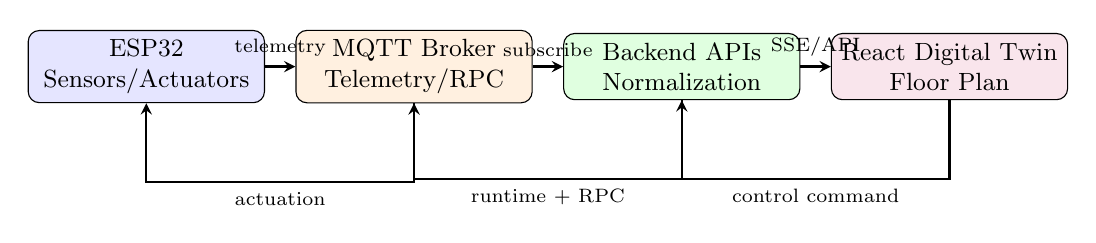
\begin{tikzpicture}[
            box/.style={draw, rounded corners, minimum width=3.0cm,
                    minimum height=0.78cm, align=center, font=\small},
            arrow/.style={->, >=stealth, thick}
        ]
        \node[box, fill=blue!10] (esp) at (0,0) {ESP32\\Sensors/Actuators};
        \node[box, fill=orange!12] (mqtt) at (3.4,0) {MQTT Broker\\Telemetry/RPC};
        \node[box, fill=green!12] (backend) at (6.8,0) {Backend APIs\\Normalization};
        \node[box, fill=purple!10] (react) at (10.2,0) {React Digital Twin\\Floor Plan};

        \draw[arrow] (esp) -- node[above, font=\scriptsize] {telemetry} (mqtt);
        \draw[arrow] (mqtt) -- node[above, font=\scriptsize] {subscribe} (backend);
        \draw[arrow] (backend) -- node[above, font=\scriptsize] {SSE/API} (react);
        \draw[arrow] (react.south) -- ++(0,-1.0) -| node[pos=0.25, below, font=\scriptsize] {control command} (backend.south);
        \draw[arrow] (backend.south) -- ++(0,-1.0) -| node[pos=0.25, below, font=\scriptsize] {runtime + RPC} (mqtt.south);
        \draw[arrow] (mqtt.south) -- ++(0,-1.0) -| node[pos=0.25, below, font=\scriptsize] {actuation} (esp.south);
    \end{tikzpicture}
    \caption{Bidirectional synchronization between the physical house and the digital twin.}
    \label{fig:digital-twin-dataflow}
\end{figure}

\subsection{Telemetry Freshness and Command Confirmation}

A digital twin is only useful when it distinguishes current state from stale state. The implementation defines a telemetry stale window of 30 seconds. If the latest telemetry timestamp is missing or older than this threshold, the floor-plan interface displays a stale-data notice and disables controls. This behavior prevents the dashboard from acting as if it knows the current physical state when the device has stopped reporting.

The command path also includes confirmation behavior. After a user toggles a marker, the frontend records the expected state and waits for telemetry to confirm that the marker reached that state. If confirmation does not arrive within the command confirmation timeout, the interface reports that the MQTT command was sent but not confirmed. This is an important digital-twin property: the visual map is updated based on observed telemetry, not merely on optimistic UI assumptions.

\subsection{Relationship with the AI Layer}

The digital twin and the multi-agent AI layer share the same device vocabulary. The AI Device Control Agent maps natural language to runtime targets, while the digital twin maps visual markers to the same targets. This shared vocabulary keeps chat control and map control consistent. For example, the user's phrase ``living room light'' and the floor-plan marker in the living room both resolve to \texttt{main\_led}. Similarly, ``bedroom light'' and the bedroom LED marker both resolve to \texttt{neo\_led}.

This common grounding model is important for thesis-level architecture because it shows that H.E.R.A is not a collection of disconnected interfaces. The dashboard, AI assistant, MQTT runtime, and firmware all refer to the same canonical device targets. The digital twin is therefore the spatial visualization layer of the same cyber-physical system described in the AI and MQTT sections.

\subsection{Design Benefits}

The implemented digital twin provides four practical benefits:

\begin{itemize}[leftmargin=*, itemsep=2pt]
    \item \textbf{Spatial interpretability:} residents can understand system state by room and object rather than by raw telemetry keys.
    \item \textbf{Unified control path:} map interactions and AI commands both use backend runtime APIs and MQTT actuation.
    \item \textbf{Telemetry-grounded visualization:} the visible state of each marker is derived from live data, not from local UI assumptions.
    \item \textbf{Failure awareness:} stale telemetry and unconfirmed commands are surfaced explicitly instead of being hidden from the user.
\end{itemize}

These properties make the floor-plan dashboard a functional digital twin of the H.E.R.A house. It continuously mirrors the physical environment, exposes room-level state, and provides a controlled path for sending actions back to the physical system.
